\documentclass{report}

% Packages
\usepackage[utf8]{inputenc}

\usepackage{amssymb}
\usepackage{amsmath}
\usepackage{amsthm}
\usepackage{pgfplots}
\newtheorem{Example}{Example}
\usepackage[T1]{fontenc}    % Encodage des polices
\usepackage[english,french]{babel} % Langue du document
\usepackage{subcaption}
\usepackage{hyperref}       % Pour les liens hypertextes
\usepackage{listings}
\usepackage{xcolor}

% Titre du rapport
\title{The Discovery of an  Algebraic structure}
\author{ASSIGBE Komi \\ RAHOUTI Chahid .}
\date{\today}

\begin{document}

\maketitle
\newpage
\tableofcontents

\newpage

\section{Introduction}


     In continuation of what we said perviously, and in this regard we are going
        to explore the algebraic structures that can be found in datasets. That is 
        through  the use of neural networks and optimization algorithms, we aim to
        discover the underlying algebraic properties of structured surfaces or 
        varieties. This project is motivated by the need to identify and characterize
        the algebraic structures inherent in datasets, which can provide valuable
        insights for data analysis and interpretation. By leveraging the power of
        neural networks and optimization techniques, we seek to uncover the 
        mathematical relationships and patterns that govern the data, enabling us to
        make predictions and draw meaningful conclusions from the dataset. This is 
        what empowers us in the future to find solutions to a group of problems that 
        addresses this project. \\ 
        In our study of this problem, we will answer a set of questions, which are as 
        follows:
        \begin{enumerate}
            \item understanding and absorbing the first algorithms that the professor developed and developed in ordre to keep up with a set of games that are based on the different dataset. 
            \item Modify the code such that we learn $\left(\oplus_\theta, \odot_\theta, f_\theta, f_\theta^i\right)$ such that
            $$
            \left\|X_i \oplus_\theta X_j-f_\theta\left(f_\theta^{-1}\left(X_i\right)+f_\theta^{-1}\left(X_j\right)\right)\right\|_{R^2}^2+\left\|\alpha_k \odot_\theta X_i-f_\theta\left(\alpha \cdot f_\theta^{-1}\left(X_i\right)\right)\right\|_{R^n}^2 \rightarrow 0
            $$
            \item Add a class mulscalaire in base . py which leans $\odot_\theta$
            \item Generate a curve in $2 \mathrm{D}$ as a dataset, we can imagine $\mathcal{M}$ as $(x, x+\varepsilon \sin (x))$ with $\varepsilon \rightarrow 0$
            \item Learn this curve to get $\left(\oplus_\theta, \odot_\theta, f_\theta, f_\theta^i\right)$
            \item Check if it sounds OK : apply $f_\theta^i$ to some (preferably unknowns) points on $\mathcal{M}$ and verify that it looks line a straight line ?
        \end{enumerate}




        % -----------------------------------------------------
        \section{Base algorithms}
        The first algorithms that the professor developed contain 
        a set of class and functions that are used to define the
        algebraic structure of a group. These algorithms are
        implemented in Python using the Pytorch library. The
        main classes and functions are as follows:

        \begin{enumerate}
            \item \textbf{Morphism}: This class defines a morphism from 
            $\mathbb{R}^n$ to a space $E$ with dimension $dim_E$. 
            It consists of three fully connected layers, each with 
            a specified number of neurons. The forward function computes 
            the output of the morphism given an input $x$.
            \item \textbf{InverseMorphism}: This class defines an inverse
            of function $f: E \rightarrow \mathbb{R}^n$. It consists of
            three fully connected layers, each with a specified number
            of neurons. The forward function computes the output of the
            inverse morphism given an input $x$.
            \item \textbf{LoiBinaire}: This class defines a binary operation 
            between two elements $x$ and $y$ in $E$. It consists of three 
            fully connected layers, each with a specified number of neurons. 
            The forward function computes the output of the binary operation 
            given two inputs $x$ and $y$.

        \end{enumerate}
        This three classes are the base of the algorithms that 
        we are going to use in our project. They are used to 
        define the algebraic structure of a group, including
        the morphism, inverse morphism, and binary operation
        between elements in a space $E$. This algorithms are used to 
        modelese the principle problem consist of finding a relation 
        between the binary operation and the morphism and the inverse
        morphism  defind by let consider a set of points  $ V $ and let 
        $ f: R \rightarrow V $ a one-to-one function from $R$ into a 
        codomain $V$. We define the binary operations $\oplus$ by
        $$ 
        x \oplus y = f(f^{-1}(x) + f^{-1}(y)) 
        $$ 
         by using the neural network.\\
        \section{Developed Code }
        In this part we are going to develop the code such as to learn 
        the two basic relations in this problem. The first relation is
        the binary operation $\oplus$ represent in $ x \oplus y = f(f^{-1}(x) + f^{-1}(y)) $  
        and the second one represent the scalar multiplication $\odot$
        $\alpha \odot x = f(f^{-1}(x) * \alpha) = \alpha x$. So we are going 
        to learn the loss of the fisrt one can be write by this formula
        $ \left\|X_i \oplus_\theta X_j-f_\theta\left(f_\theta^{-1}\left(X_i\right)+f_\theta^{-1}\left(X_j\right)\right)\right\|_{R^2}^2 $  
        and the loss of the second one can be write by this formula
        $ \left\|\alpha_k \odot_\theta X_i-f_\theta\left(\alpha \cdot f_\theta^{-1}\left(X_i\right)\right)\right\|_{R^n}^2 $
        in order to minimize the loss function we are going to use the 
        Pytorch library in Python using Neural Networks Learning to find
        the optimal parameters that minimize the loss function.
        After to defined this two losses we learn the sum between them by this
        formula 
        $$
            \left\|X_i \oplus_\theta X_j-f_\theta\left(f_\theta^{-1}\left(X_i\right)+f_\theta^{-1}\left(X_j\right)\right)\right\|_{R^2}^2+\left\|\alpha_k \odot_\theta X_i-f_\theta\left(\alpha \cdot f_\theta^{-1}\left(X_i\right)\right)\right\|_{R^n}^2 \rightarrow 0
        $$ 
        If this quantity is converging to zero, we can say that the model 
        is learning the two relations.\\


        \section{Analysis and interpretation}
        We are going to analyze this two losses by defining the
        class Mulscalaire in the base.py file and taking  a set of data to 
        generate a curve in $2D$ as a dataset. We can imagine $\mathcal{M}$ as
        $(x, x+\varepsilon \sin (x))$ with $\varepsilon \rightarrow 0$ and comment results. We are
        going to learn this curve to get $\left(\oplus_\theta, \odot_\theta, f_\theta, f_\theta^i\right)$
        and check if it sounds OK by applying $f_\theta^i$ 
        to some (preferably unknowns) points on $\mathcal{M}$ 
        and verify that it looks like a straight line.\\

        \subsection{Class Mulscalaire}

        In this part we are going to add a class called Mulscalaire 
        in the base.py file. This class is used to define the scalar
        multiplication operation $\odot_\theta$. The class consists of
        three fully connected layers, each with a specified number of
        neurons. The forward function computes the output of the scalar
        multiplication operation given an input $\alpha$ and $x$. 



        \subsection{Dataset}
        We take a set of data to generate a curve in $2D$ as a dataset.
        and analaysis the results. We can imagine $\mathcal{M}$ as 
        $(x, x+\varepsilon \sin (x / \varepsilon))$ with $\varepsilon \rightarrow 0$.t
        this function has same ociilating behavior.
        \begin{figure}[h!]
            \centering
            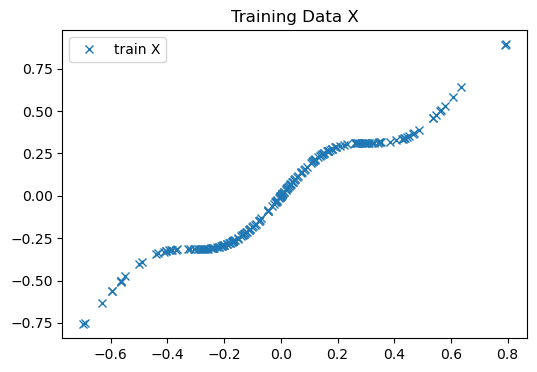
\includegraphics[width=0.5\textwidth]{curve.png}
            \caption{Curve in $2D$}
            \label{fig:curve}
            \end{figure}

        \subsection{Learning the resultat of training}
        The quantity $$
            \left\|X_i \oplus_\theta X_j-f_\theta\left(f_\theta^{-1}\left(X_i\right)+f_\theta^{-1}\left(X_j\right)\right)\right\|_{R^2}^2+\left\|\alpha_k \odot_\theta X_i-f_\theta\left(\alpha \cdot f_\theta^{-1}\left(X_i\right)\right)\right\|_{R^n}^2 \rightarrow 0
        $$ is converging to zero, we can say that the model is learning the two relations.\\
        We see this results for exmple if x between $ 0 $ and $ 1 $ we have the following results
        \begin{table}[h]
            \centering
            \begin{tabular}{|c|c|c|c|}
            \hline
            Epoch & Loss 1 & Loss 2 & Total Loss \\
            \hline
            0/50 & 36.229023 & 48.668434 & 84.897461 \\
            10/50 & 0.243487 & 1.066152 & 1.309639 \\
            20/50 & 0.035945 & 0.227918 & 0.263863 \\
            30/50 & 0.011098 & 0.086047 & 0.097145 \\
            40/50 & 0.005786 & 0.023966 & 0.029752 \\
            \hline
            \end{tabular}
            \caption{Training results with 64 neurons per layer}
            \label{tab:training_results}
            \end{table}
    We can see that the total loss is converging to zero as the number of epochs increases, 
    indicating that the model is learning the two relations. This is a good sign that the
    model is able to capture the underlying algebraic structure of the dataset.\\
    \subsection{Interpretation}
    We can interpret the results by applying $f_\theta^i$ to some points on $\mathcal{M}$
    and verifying that it looks like a straight line. This will help us to understand 
    how well the model has learned the two relations and whether it is able to capture
    the underlying algebraic structure of the dataset.
    This is the results of the training 
    \begin{figure}[h!]
        \centering
        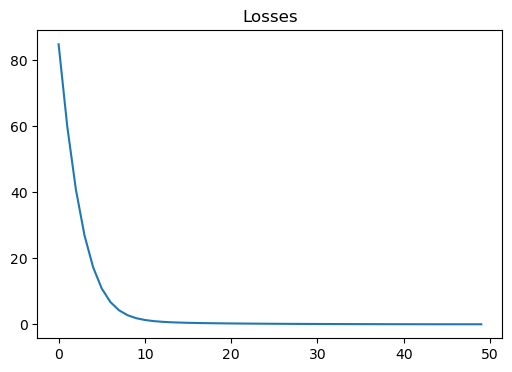
\includegraphics[width=0.5\textwidth]{optim.png}
        \caption{Losses}
        \label{fig:losses}
        \end{figure}
    This is the results of the output and interpetation of resulat is a straight line
        \begin{figure}[h!]
            \centering
            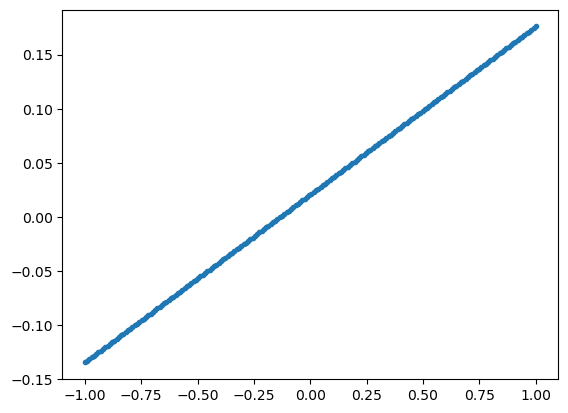
\includegraphics[width=0.5\textwidth]{output.png}
            \caption{Output}
            \label{fig:straight}
            \end{figure}


    \section{Conclusion}
    In this project, we have explored the algebraic 
    structures that can be found in datasets and
    how they can be effectively learned using
    neural networks and optimization algorithms.
    This results can be said is good bath this result in 
    $R^n$ all of that will bring us to an important question,
    which is how we can modelese this two relation in whatever varieties.


    
\end{document}